\section{Methodology and Dataset}
\label{sec:Methodology}

We used \platname to characterize mobile Internet traffic, specifically, we detail the impact of mobile applications, access technology, and operating systems on mobile Internet traffic.

Our analysis methodology included controlled experiments to detail the behavior of specific applications and OS services, and a 7-month long IRB approved measurement study to characterize mobile Internet traffic in the \emph{in the wild}.

\subsection{Controlled Experiments}

For our controlled experiments, we ran the latest versions of Android (Ice Cream Sandwich 4.0, and Jelly-bean 4.2) and iOS 6 respectively on our Android and iOS devices. 
We analyze the behavior of OS services and the default applications by first performing a factory reset on these devices, and installing the \platname credentials on this device.
We then test Android and iOS applications by installing the application, interacting with the application for a few minutes, and finally uninstalling the  application. 
During our controlled experiment we use SSL-Bumping to study the behavior of SSL traffic from these applications. 

Our first experiment included manual testing of the top 100 most popular free Android apps from the \emph{Google Play} store and \tbd{} iOS applications from the iOS App store.
During this experiment, for each application, we enter user credentials for accounts like Facebook and Twitter, and toy with the app for \tbd{} minutes. 

For our second experiment we performed fully-automated tests on 1003 Android applications from a free, third-party Android market.
We perform this test because Android devices can install \emph{Third-party applications} that are not available on the \emph{Google Play} store.
A consequence of this freedom is that numerous third-party app markets are available on the web whose applications have not received research attention.
For our automation we used adb Android command shell to install each app, enable \platname, and start the app.
We then used Monkey, an adb stress tool, to perform a series of 10,000 actions which includes random swipes, touches, and text entries.
We then used adb to uninstall the application and reboot the device to forcibly end any lingering connections.

The results of our controlled experiments can be found in \fref{sec:manual-testing}.

\subsection{In The Wild Measurements}

Along with controlled experiments we also conducted an IRB approved measurement study to characterize the mobile Internet in the wild.
We now present the description of the dataset and the methodology we used to classify the traffic in this dataset.

For this study, we deployed two \platname servers, one in USA and one in France, to proxy Internet traffic from 26 devices, 10 iPhones, 4 iPads, 1 iPodTouch, and 11 Android phones.
The Android devices in this dataset include the Nexus, Sony, Samsung, and Gsmart brands while the iPhones include one iPhone~3gs, five iPhone~5, and five iPhone~4S.
These devices belonged to 21 users, volunteers for our IRB approved study.
This dataset, called \mobWild, consists of 218 days of data that flowed through our \platname servers; the number days for each user varies from 5 to 215 with a median of 35 days.
We would like to point out that though we performed SSL-Bumping during our controlled experiments, we did not perform SSL-Bumping for the traffic in this dataset.

Capturing all of a subject's Internet traffic raises significant privacy concerns. 
Our IRB-approved study entails informed consent from subjects who are interviewed in lab, where the risks and benefits of our study are clearly explained. 
The incentive to use VPNs was a lottery of Amazon.com gift certificates
To protect the identity of information leaked in the data, we use public key cryptography to encrypt all the tcpdump outputs; the private key is maintained on separate secure severs and with access limited to approved researchers. 
Furthermore, user are free to delete their data and/or disable monitoring at any time. 
For privacy reasons, we cannot make this data publicly available.



%%% Local Variables: 
%%% mode: latex
%%% TeX-master: "main"
%%% End: 

% We used Bro~\cite{bro} to analyze the traffic the passed through our \platname servers.
% In \fref{tab:summaryIOSAndroidTraffic} we summarize \mobWild based on the classification performed using Bro~\cite{bro}.
% Bro classifies IP flows using the protocol field in the IP header.
% We use this classification to label flows as either TCP, UDP, or \emph{other}; flows that are neither TCP nor UDP are classified as \emph{other}. 
% Bro further uses the well defined port numbers to identify the services that use TCP.
% We use this classification to label flows as either HTTP, SSL (which includes HTTPS, IMAP, etc.) or \emph{other} flows; TCP flows that are not classified as either HTTP or SSL are classified as \emph{other}.
% In \fref{tab:summaryIOSAndroidTraffic}, we observe that more than 90\% of the traffic in our dataset is either HTTP or SSL. 
% We also observe that the share of HTTP volume over \wifi and cellular are significantly different. 
% As detailed in \fref{sec:.}, this difference is primarily due to the use of \wifi to transfer media content.
% We also observe the share of SSL traffic over cellular networks is considerably larger compared to \wifi networks.
% This increase is a result of the reduced share of media traffic and the use of email and for social networking applications that rely on SSL.
% We detail the HTTP and SSL traffic from iOS and Android devices in \fref{sec:}

% We focus our application classification on TCP because TCP is responsible for than 90\% of the traffic volume in our dataset (see~\fref{tab:summaryIOSAndroidTraffic}).
% \begin{figure}
% 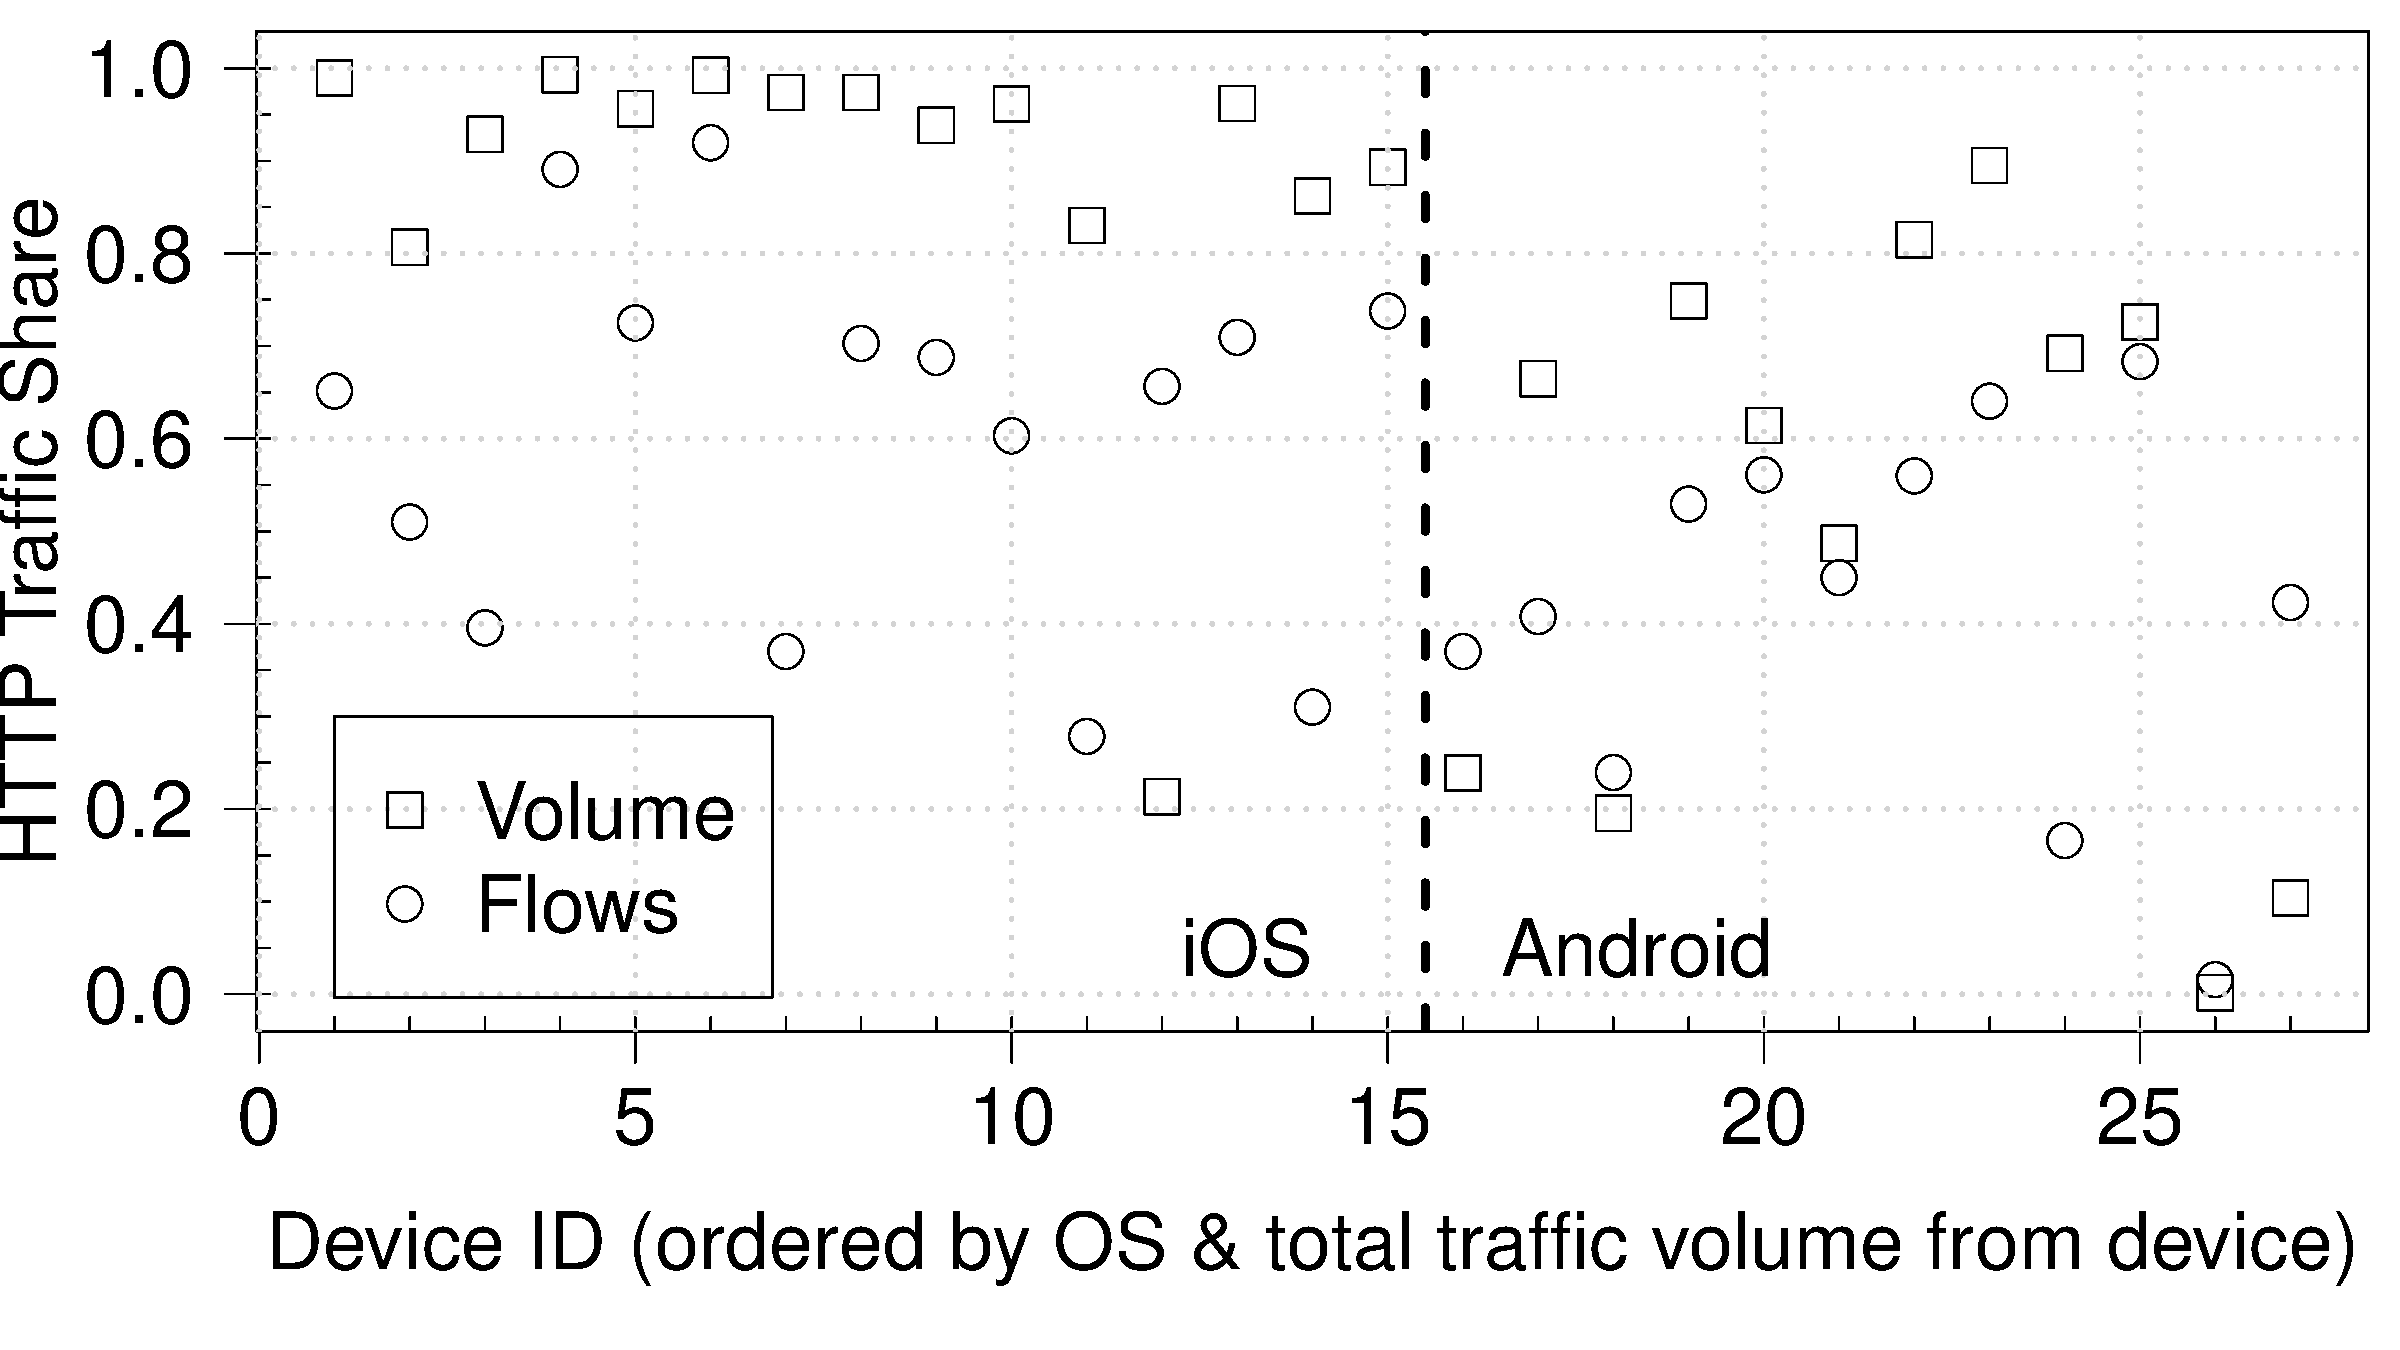
\includegraphics[width=\columnwidth]{plots/appusage_someappsig_traffic.pdf}
% \caption{HTTP traffic with a \useragent field containing an identifier of an application (other than Web-browser) or an OS service. 
% \emph{A smaller share of Android HTTP traffic can be classified using User-Agents because Android applications are not limited to underlying OS media services such as AppleCoreMedia.}}
% \label{fig:http-classification-app-user-agent}
% \end{figure}

% In \fref{fig:http-classification-app-user-agent} we plot the fraction of HTTP traffic for we were able to identify an application signature; the devices are ordered according to the operating system, and for each operating system we further order the devices according to the total traffic from the device that flowed through \platname. 
% We observe that a significantly larger fraction of traffic from iOS device can be mapped to an application in comparison to the traffic from Android devices. 
% For example, while more than 80\% of HTTP traffic from iOS devices contain an application or OS service signature in the \useragent field, only 23.9\% and 19.5\% from Android devices with id 16 and 18 contained useful signatures in the \useragent field.
% On further inspection we observe that this difference is because of the techniques used by Android and iOS application to download audio and video content. 

% \begin{figure}
% 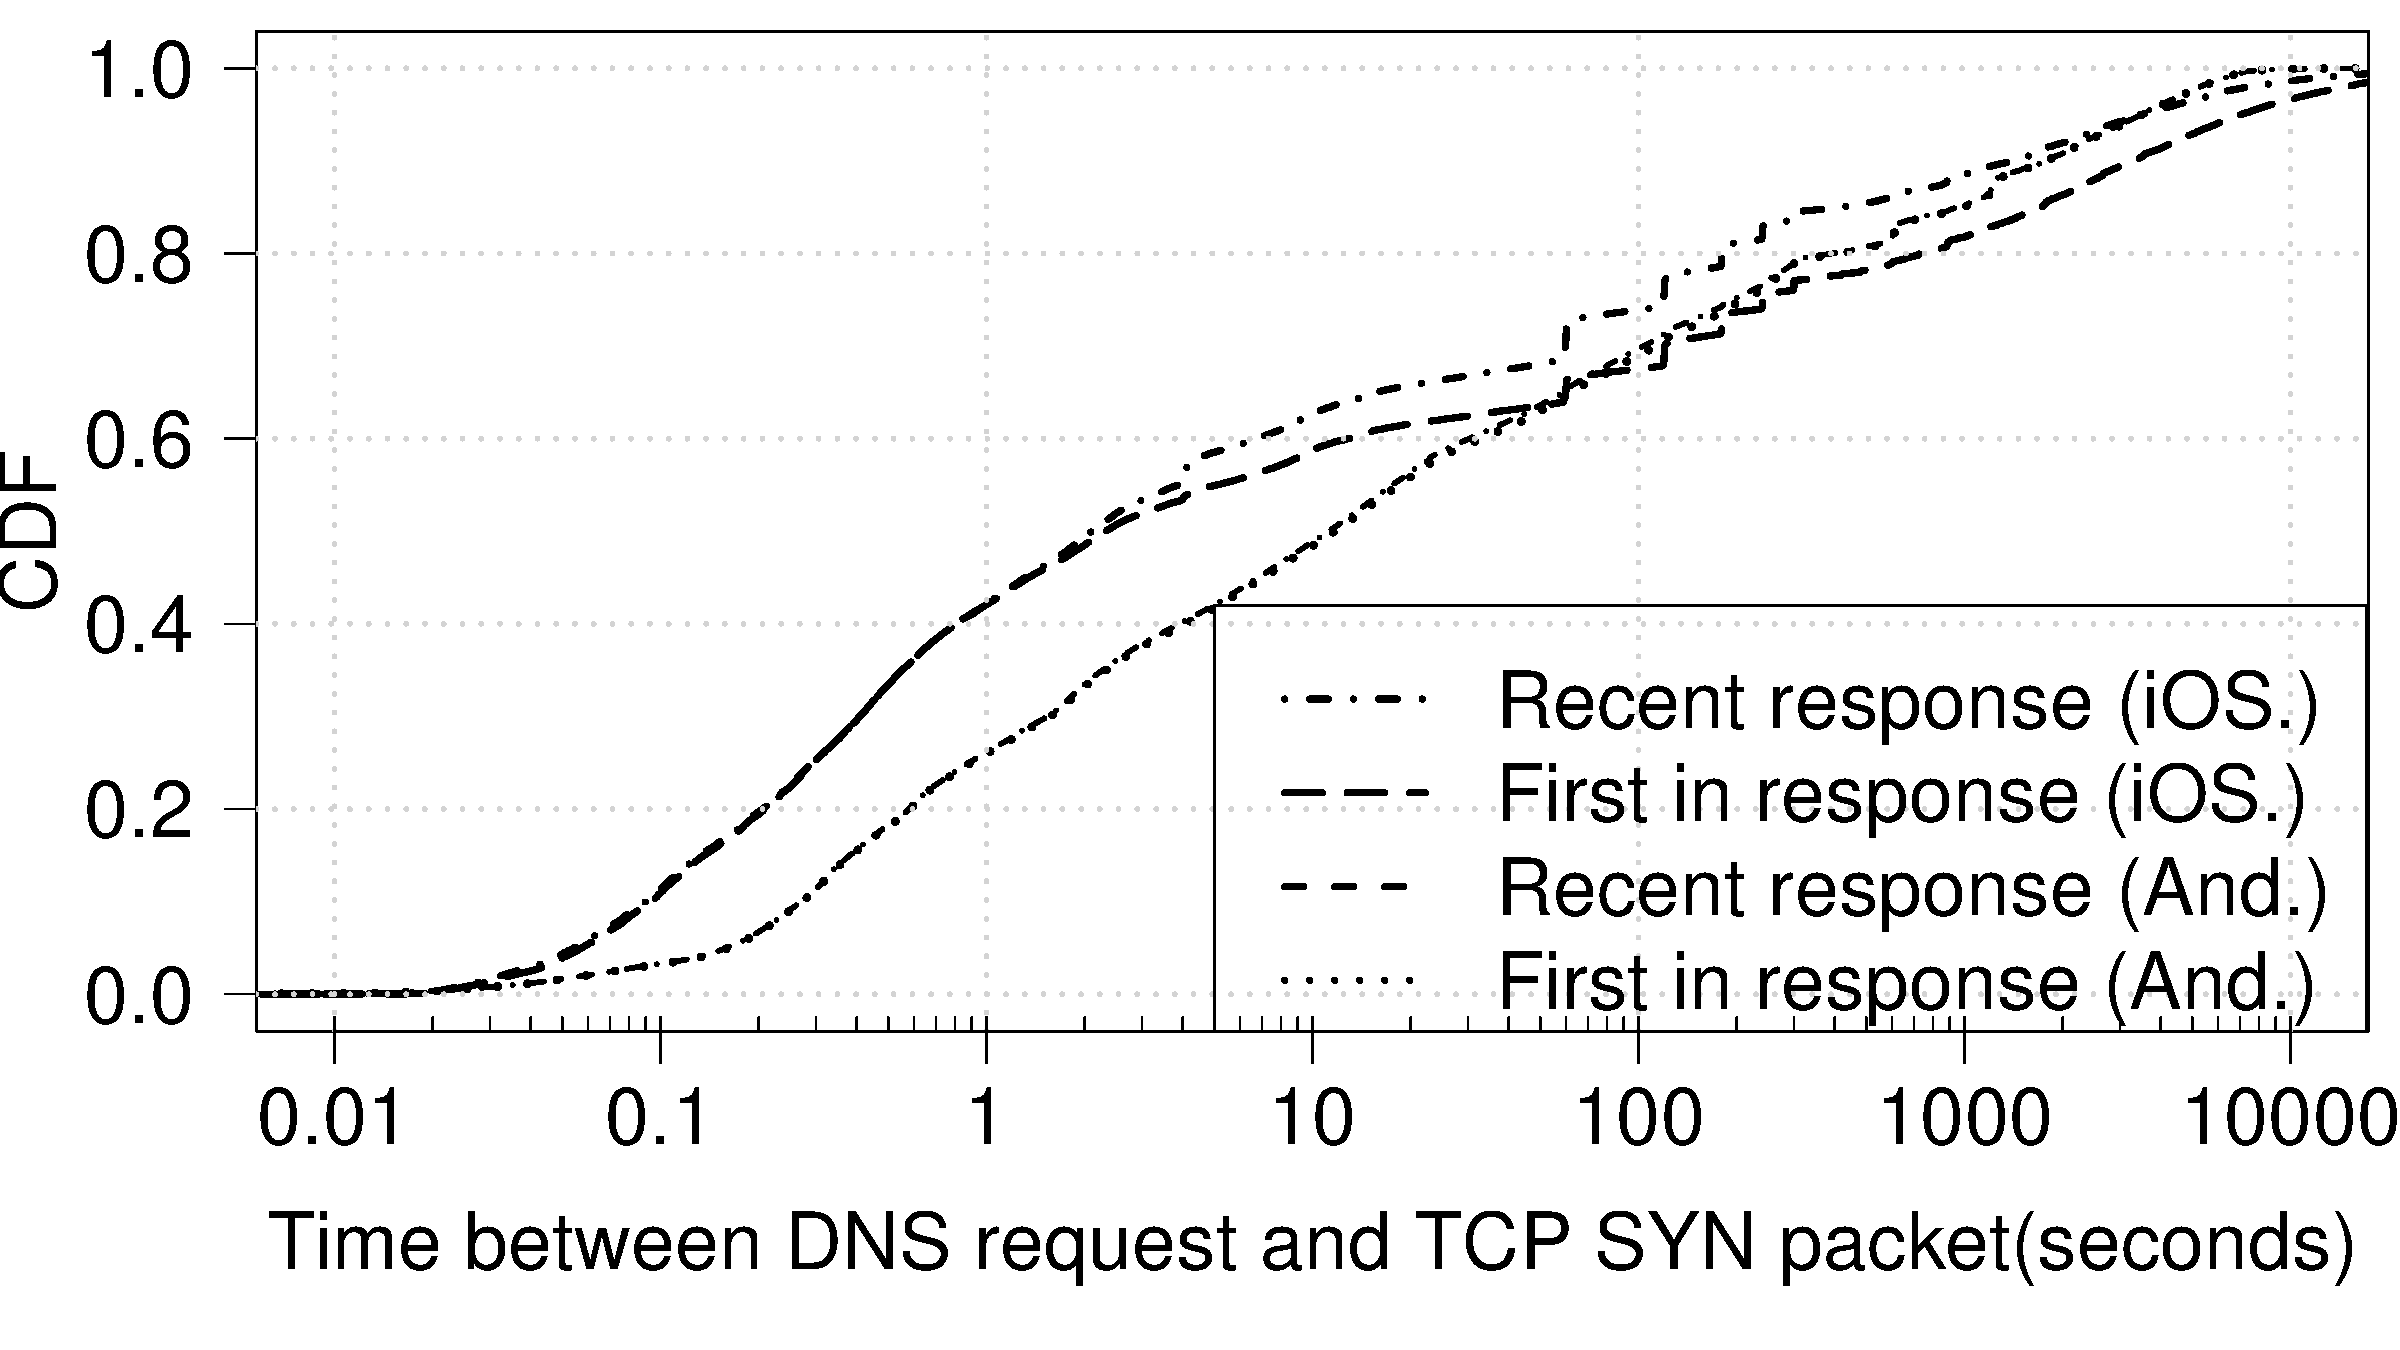
\includegraphics[width=\columnwidth]{plots/sslanalysis_dns_timediff_distrib.pdf}
% \caption{Distribution of the time between DNS response that contained the IP address of the SSL server and the SYN from the SSL flows. 
% \emph{The lack of difference in the curves for Android devices implies that the first entry in the most recent DNS response contained the IP address of the SSL flow.\tbd{rename xlab to DNS response.}}}
% \label{fig:ssl-dns-first-recent-distrib}
% \end{figure}

% To analyze the impact of the ambiguity, in \fref{fig:ssl-dns-first-recent-distrib} we plot the distribution of the time between the DNS response that contained the IP address and SYN packet from the SSL flow. 
% For this plot, we consider two types of DNS responses: the most recent DNS response that contain the IP address in the SSL flows, and the most recent DNS response that contained the IP address as the first entry in the DNS response. 
% We observe that for Android flows we do not observe a difference in the curves for the distribution, implying that the first entry in the most recent DNS response contained the IP address of the SSL flow.
% However, for iOS devices we observe a difference in the distribution when the time difference between the SYN and DNS response is larger than three seconds. 
% This difference creates an ambiguity which can be aggravated by caching of name resolution by the applications. 
